\subsection{Salient features}
\label{sec:data_features}

% As far as the color, t
The picture appearance is dominated by two prevalent tints due to the intentional selection of a specific wavelength: a darker hue corresponding to areas whose light was filtered out and a yellow tone emitted by the fluorophore
(\cref{fig:dataset:empty,fig:dataset:dark,fig:dataset:bright,fig:artifacts}).
As a consequence, the only color channels to be populated are red and green, while blue is typically empty. 
An example of this effect is reported in \cref{fig:dataset:pixel_intensity}, where the average distribution of pixel intensity is illustrated (log scale).
\begin{figure}
    \centering
    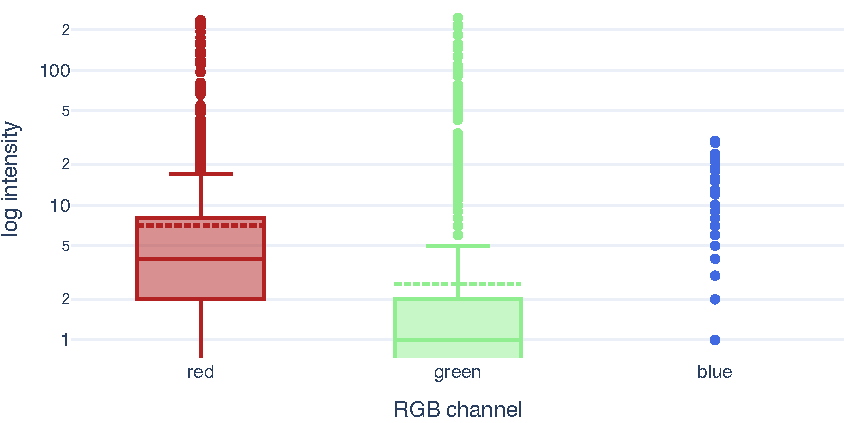
\includegraphics[width=\textwidth]{figures/120_dataset/features/pixel_intensity_distribution.pdf}
    \caption{\textbf{Pixel intensity distribution.} Violin plot of the average distribution of pixel intensities across the  RGB channels}
    \label{fig:dataset:pixel_intensity}
\end{figure}
In practice, the blues have an extremely narrow distribution squashed on zero, which makes it even difficult to visualize -- in fact only outliers are visible. 
The red and green channels are instead more populated. Their central tendency is still concentrated on low values due to the prevalence of background pixels, however we observe longer and thicker right tails, especially for the red channel (see \textit{red}, \textit{green} and \textit{blue} columns in \cref{tab:data_features} for a numeric summary).
Guided by this observation, one may argue that all this information is superfluous, so resorting to a grayscale transformation could be better since the images are ultimately shades of yellow.
A nice way to visually investigate such relationships is by exploring the colorspace representations of several images.
\Cref{fig:dataset:colorspace} reports the RGB and HSV encodings for two randomly sampled images.
Indeed, the RGB representations (\cref{fig:dataset:colorspace:rgb1,fig:dataset:colorspace:rgb2}) corroborate the previous intuition, as most pixels lay almost on a straight line in the red-green plane. 
This suggests that the two channels are highly correlated, so a one-dimensional subspace may be enough to represent most of the variability of the data.
In turn, this would bring two advantages: ease the learning process -- as neural networks typically suffer when inputs are correlated %\cite{} 
-- and make it more efficient -- as only one channel is considered instead of three.

However, the use-case at hand has no stringent requirements in terms of computing resources and runtime, so the 3-channels training is still feasible.
More importantly, the information thrown away when converting to grayscale, although tiny, may be crucial to discriminate background and signal. 
Hence, a 3D-encoding may still be worthed but the RGB colorspace may not be the optimal representation to learn this separation. A hint of that is demonstrated in \cref{fig:dataset:colorspace:hsv1,fig:dataset:colorspace:hsv2}, where the same images are depicted according to the HSV encoding. 
In this case, the separation between dark and colored tones appears more evident. 
Moreover, most of the pixels are concentrated in low hue values
and their distribution seems more spread across the saturation-value plane. 

All that being considered, we try to leverage the insights of both approaches. 
On one side, the RGB colorspace is taken as a starting point to retain all available information. On the other, the model first layer is designed to incorporate a colorspace transformation from RGB to a single channel.
% In this way, the intent is to avoid introducing any colorspace-related bias by letting the model learn the most convenient representation and, at the same time, benefit from the computational advantage due to a lower dimensionality.
% The intent is to avoid introducing any colorspace-related bias by letting the model learn the most convenient representation without ignoring the fact that a one-dimensional manifold is probably enough to express the variability of the data.
% The intent is to avoid introducing any colorspace-related bias by letting the model learn the most convenient representation.
% At the same time, by forcing the learned encoding to one dimension, we do not ignore the observation that a one-dimensional manifold is probably enough to express the data variability.
In this way, we avoid introducing any colorspace-related bias since the model learns the most convenient representation.
At the same time, we exploit the observation that a one-dimensional manifold is probably enough to express the data variability by forcing the learned encoding to one channel.
% \begin{figure}
%     \centering
%     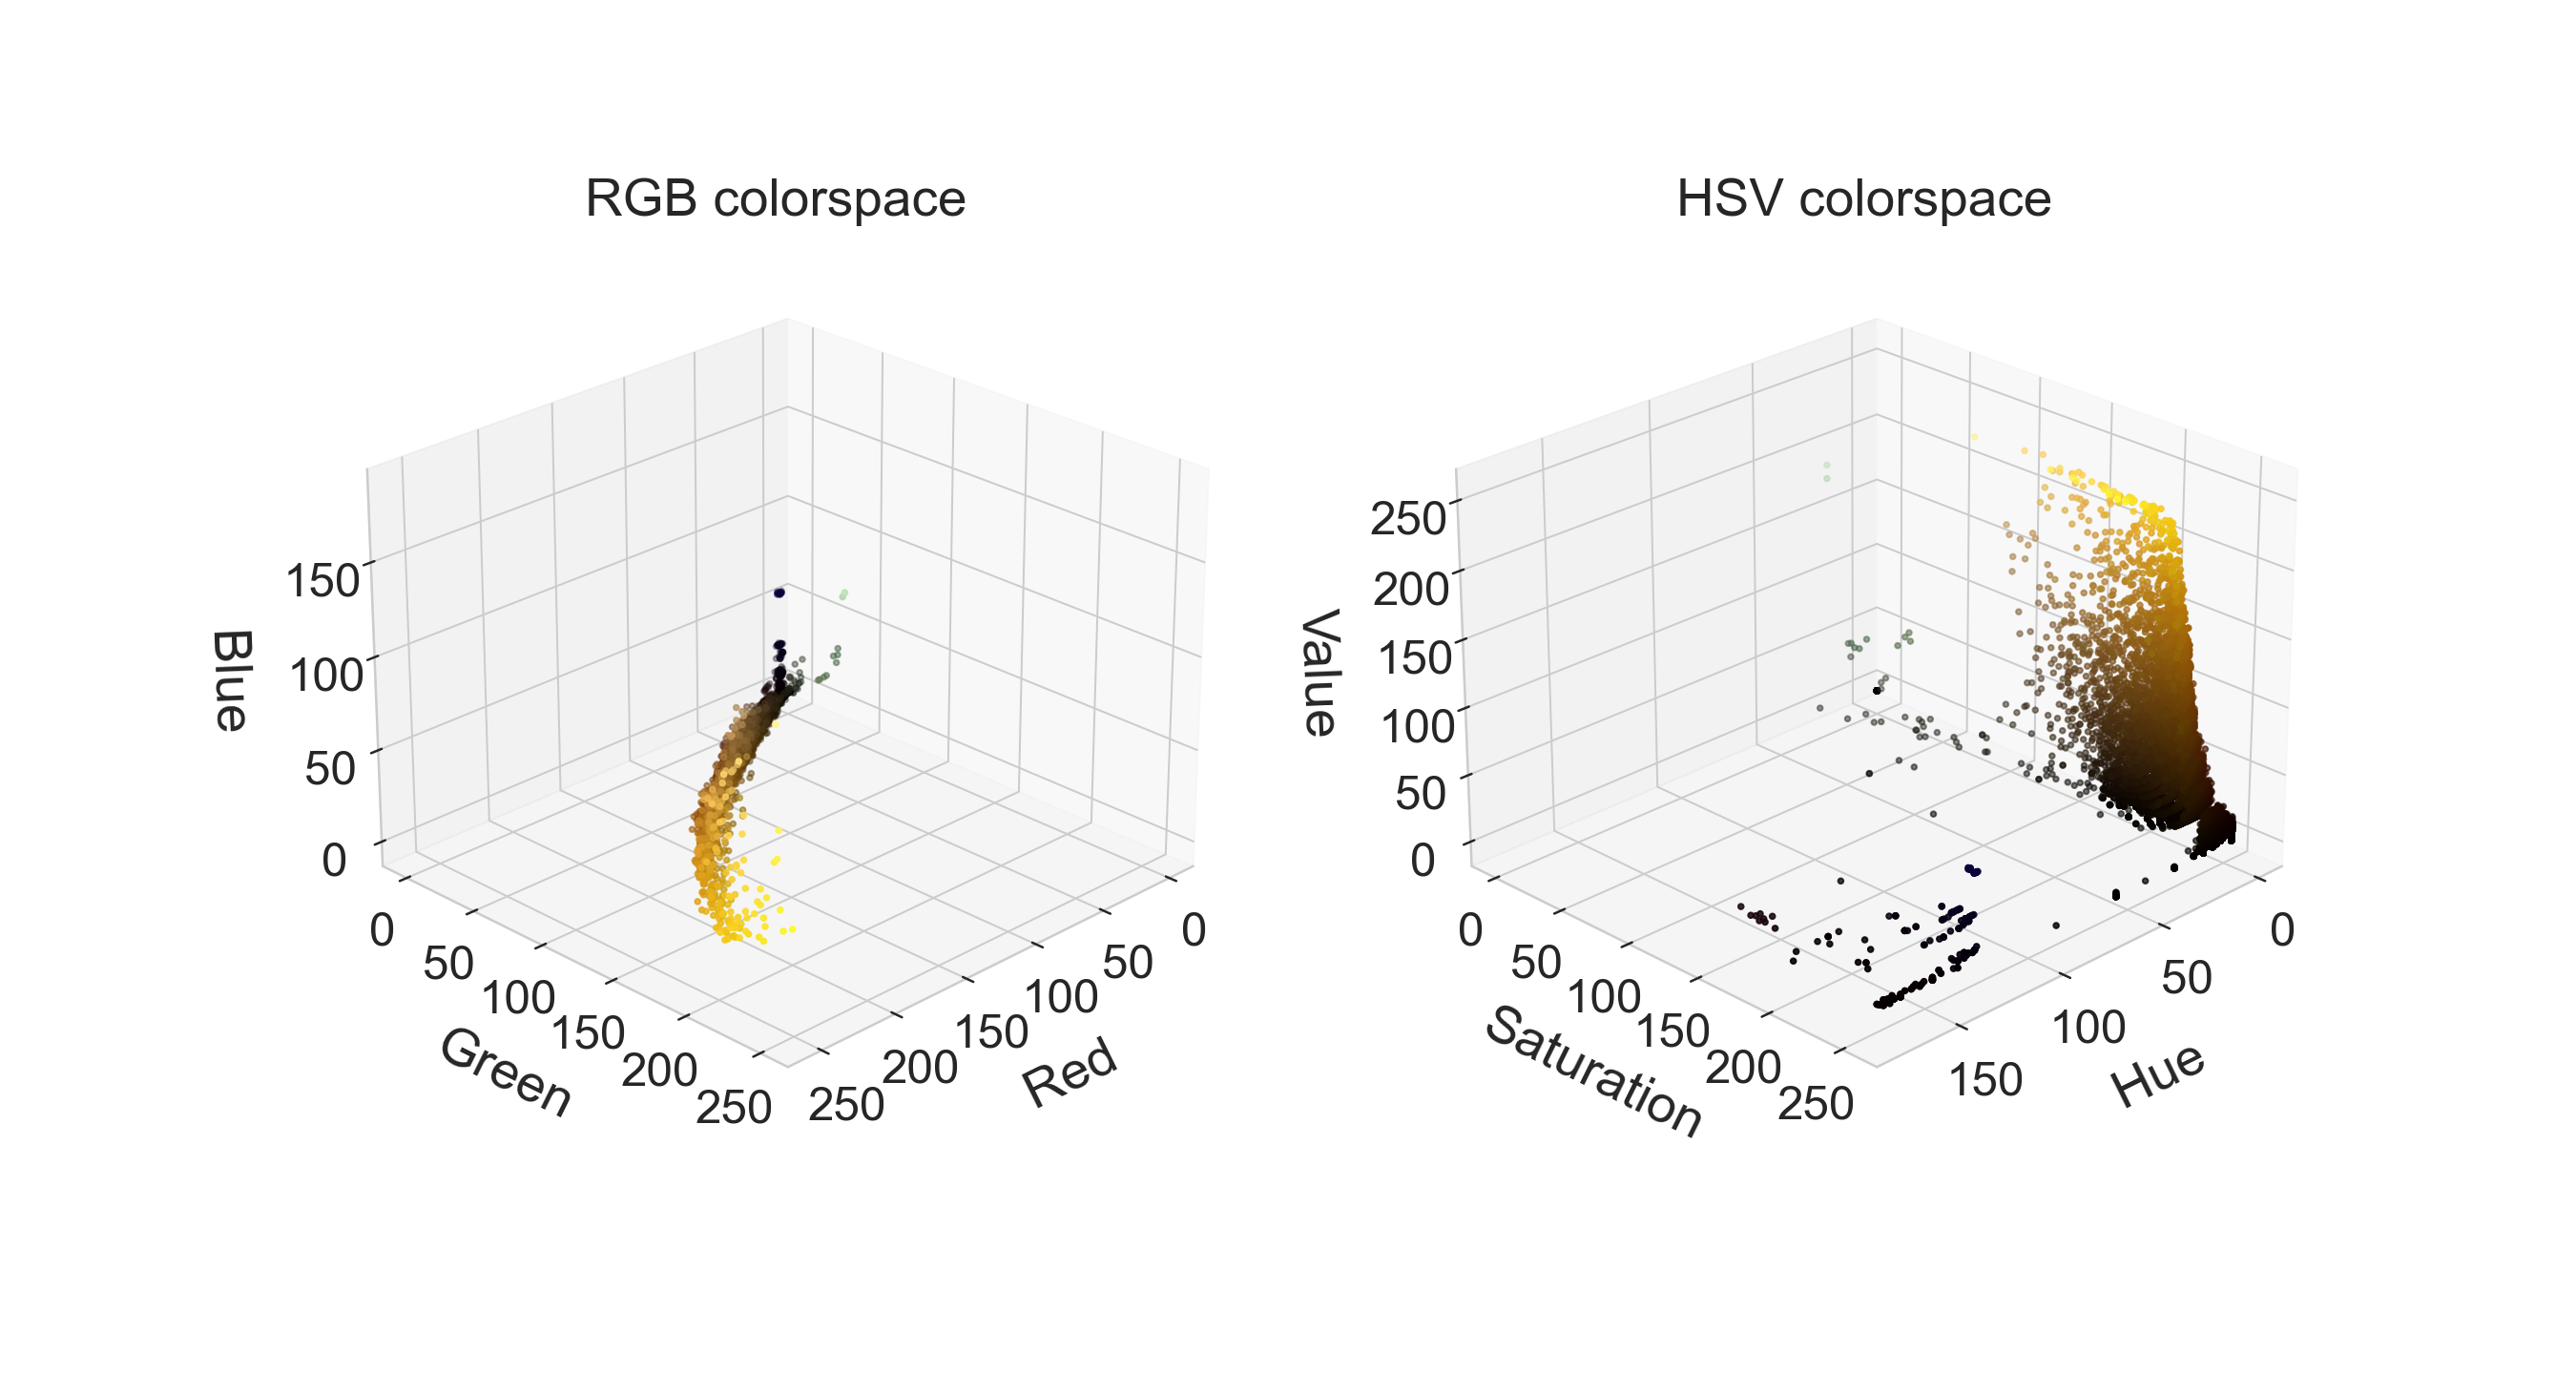
\includegraphics[width=1.1\textwidth]{figures/120_dataset/colorspace_Mar23bS1C2R3_VLPAGl_200x_y.png}
    
%     \centering
%     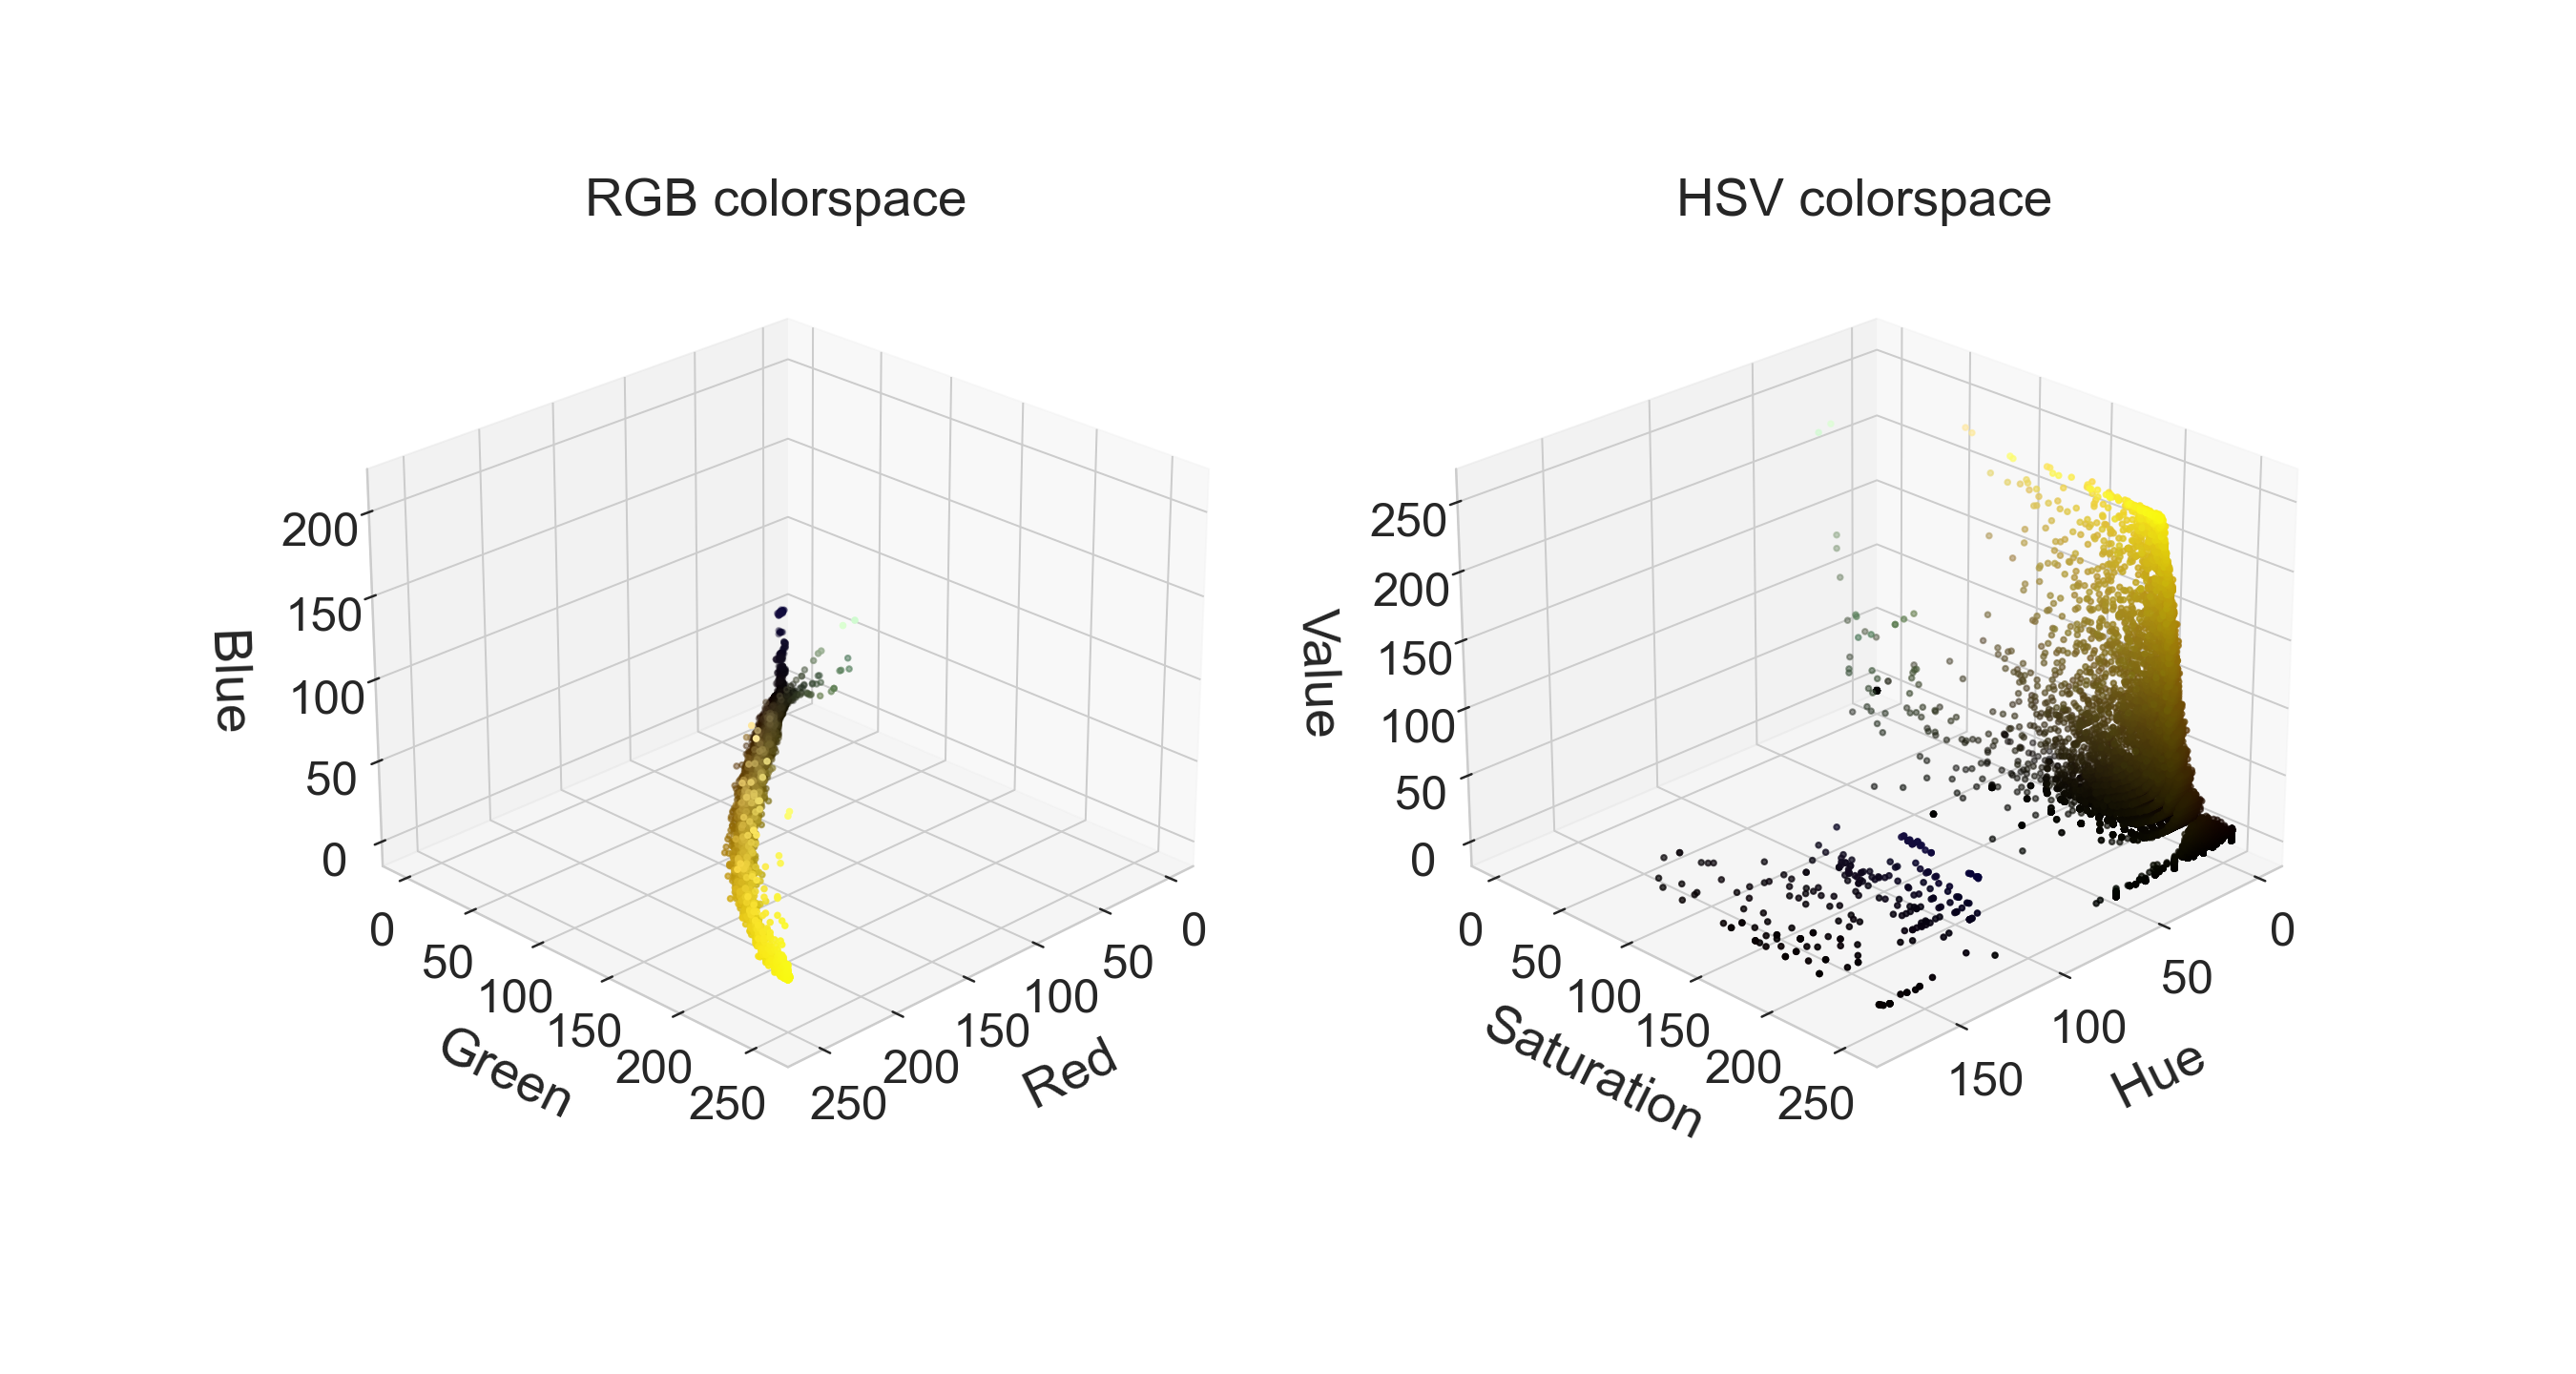
\includegraphics[width=1.1\textwidth]{figures/120_dataset/colorspace_Mar26bS2C1R2_DMl_200x_y.png}
%     \caption{Colorspace representation. The same image is represented as RGB (left) and HSV (right). Pixels are treated as 3D points with coordinates given by their encoding in the corresponding colorspace}
%     \label{fig:dataset:colorspace}
% \end{figure}
% \savegeometry{origigeom}
% \clearpage
% \newgeometry{lmargin=0.5cm}
\begin{figure}

    \centering
    Mar19bS1C4R3\_LHl\_200x\_y.png
    % \vspace{-3cm}
    \makebox[\textwidth][c]{\subfloat[RGB]{
    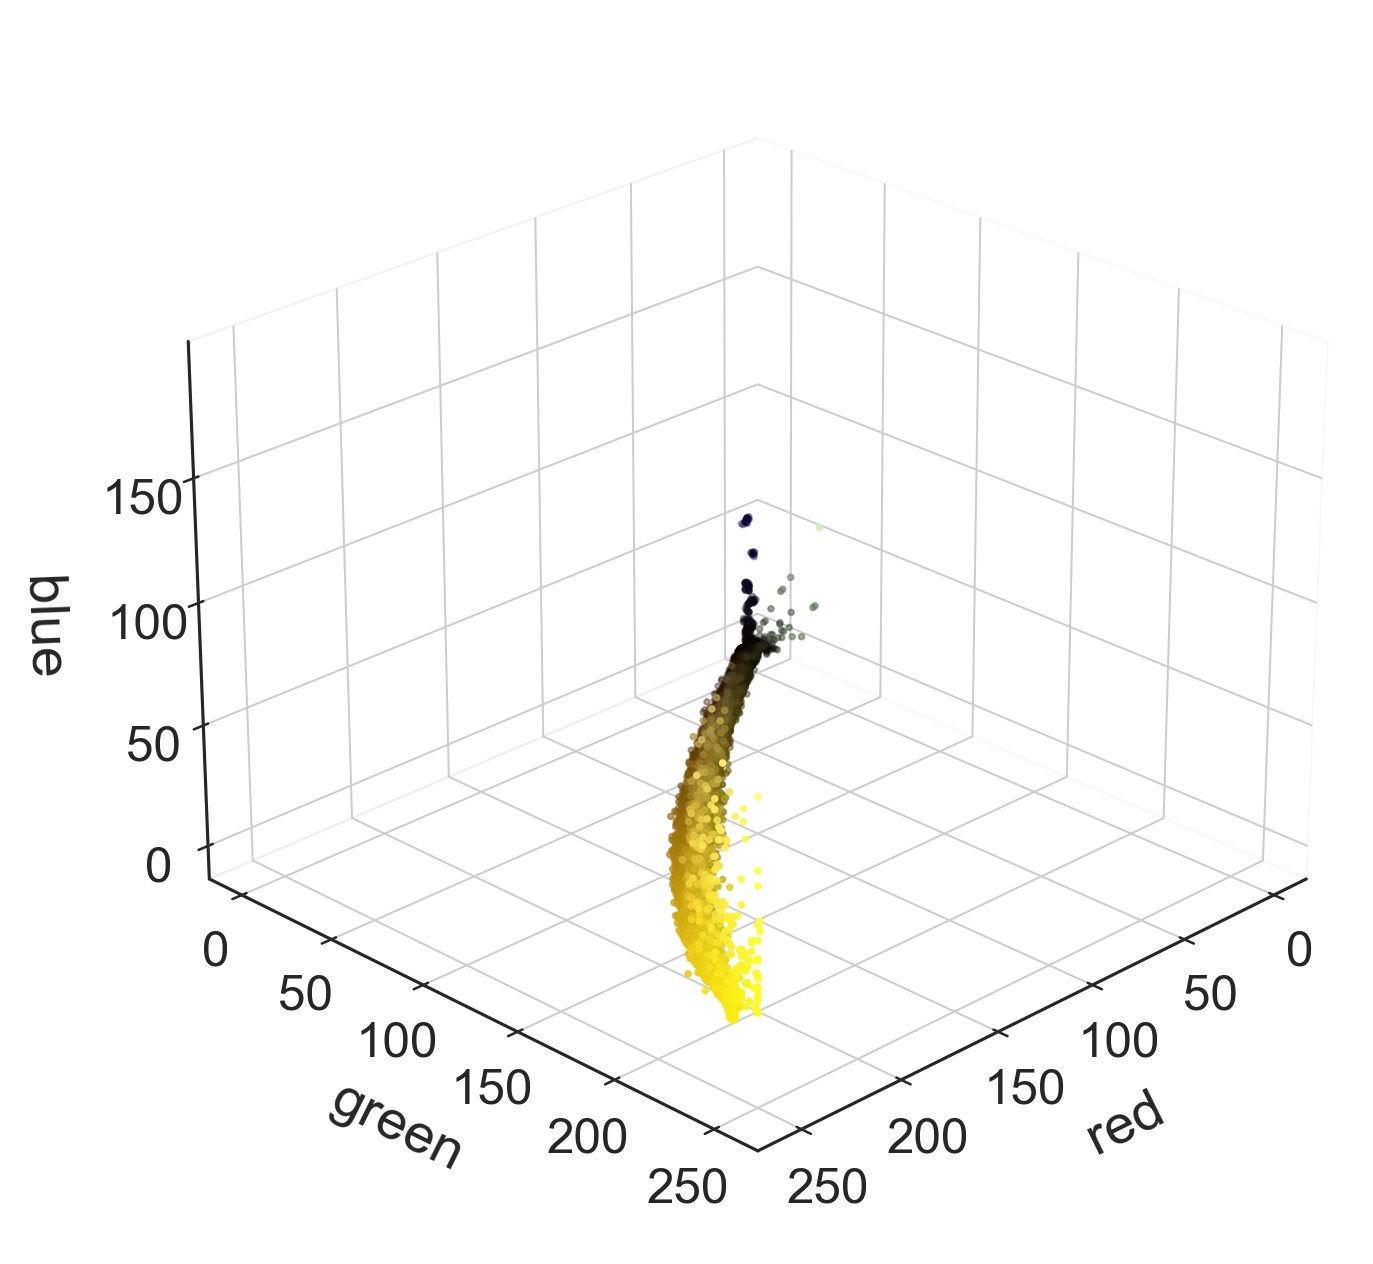
\includegraphics[width=0.55\textwidth]{figures/120_dataset/RGB_Mar19bS1C4R3_LHl_200x_y.png}\label{fig:dataset:colorspace:rgb1}
    }
    \subfloat[HSV]{
    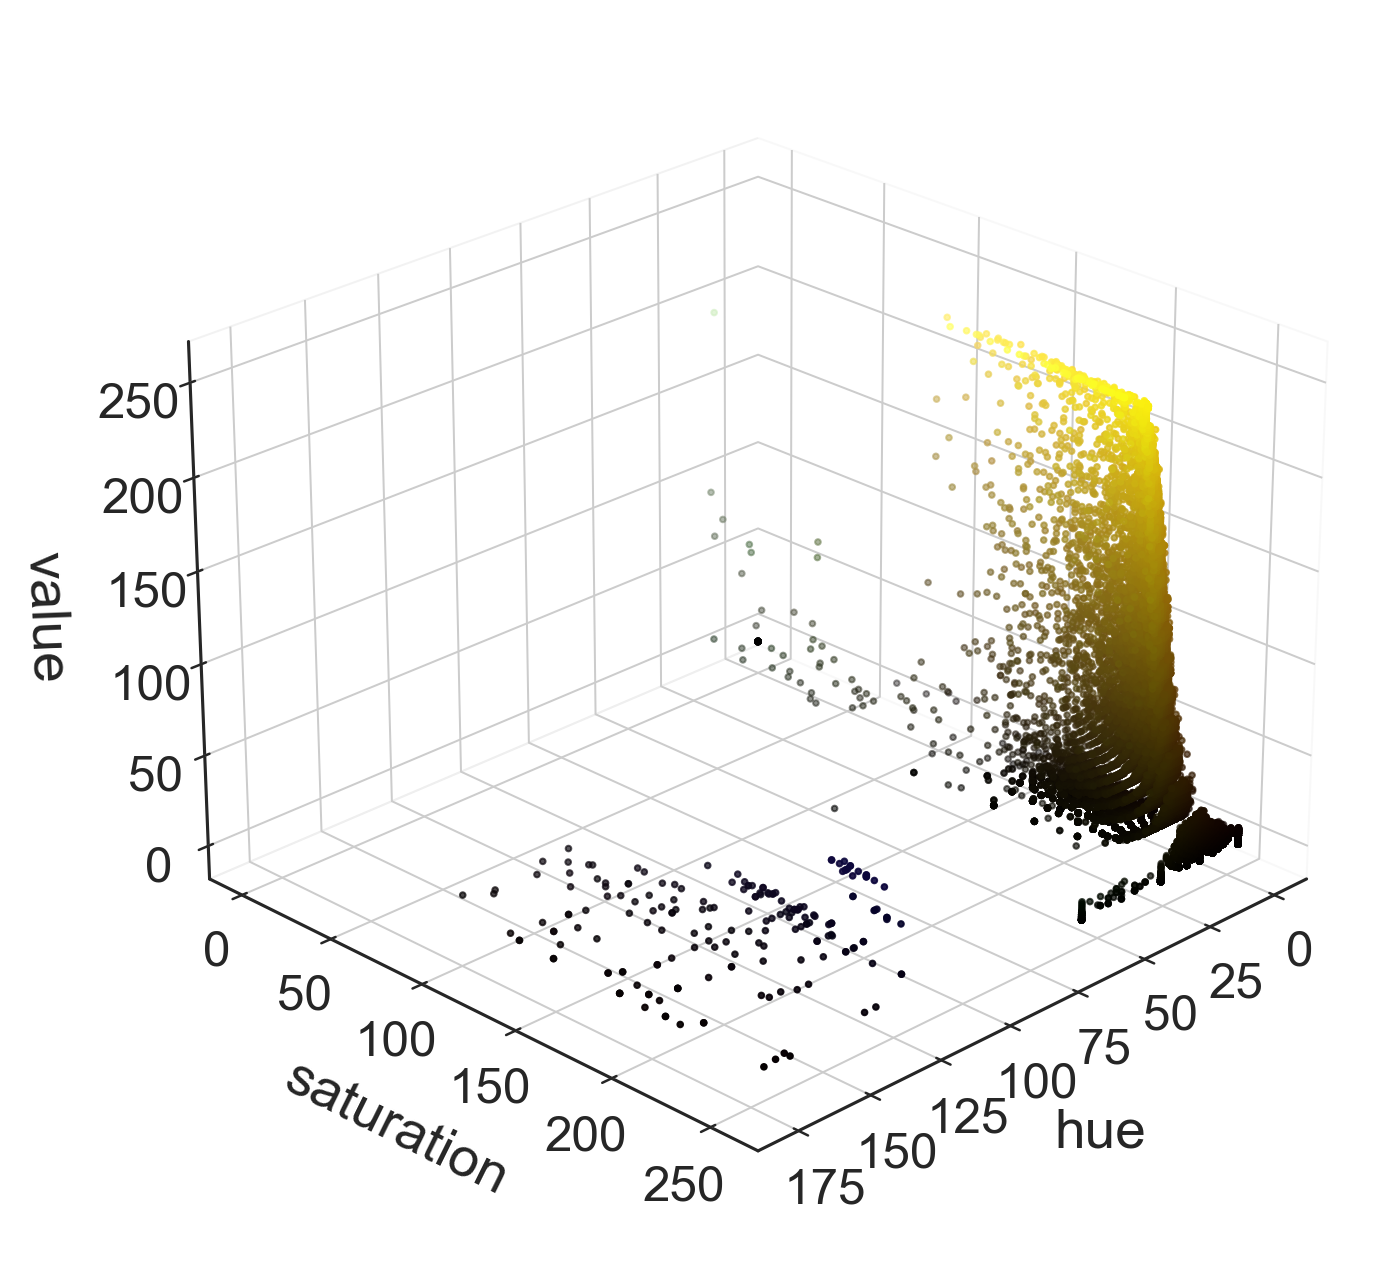
\includegraphics[width=0.55\textwidth]{figures/120_dataset/HSV_Mar19bS1C4R3_LHl_200x_y.png}\label{fig:dataset:colorspace:hsv1}
    }}
    
    \centering
    \vspace{1.5cm}
    Mar21bS1C1R3\_VLPAGl\_200x\_y.png   \makebox[\textwidth][c]{ \subfloat[RGB]{
    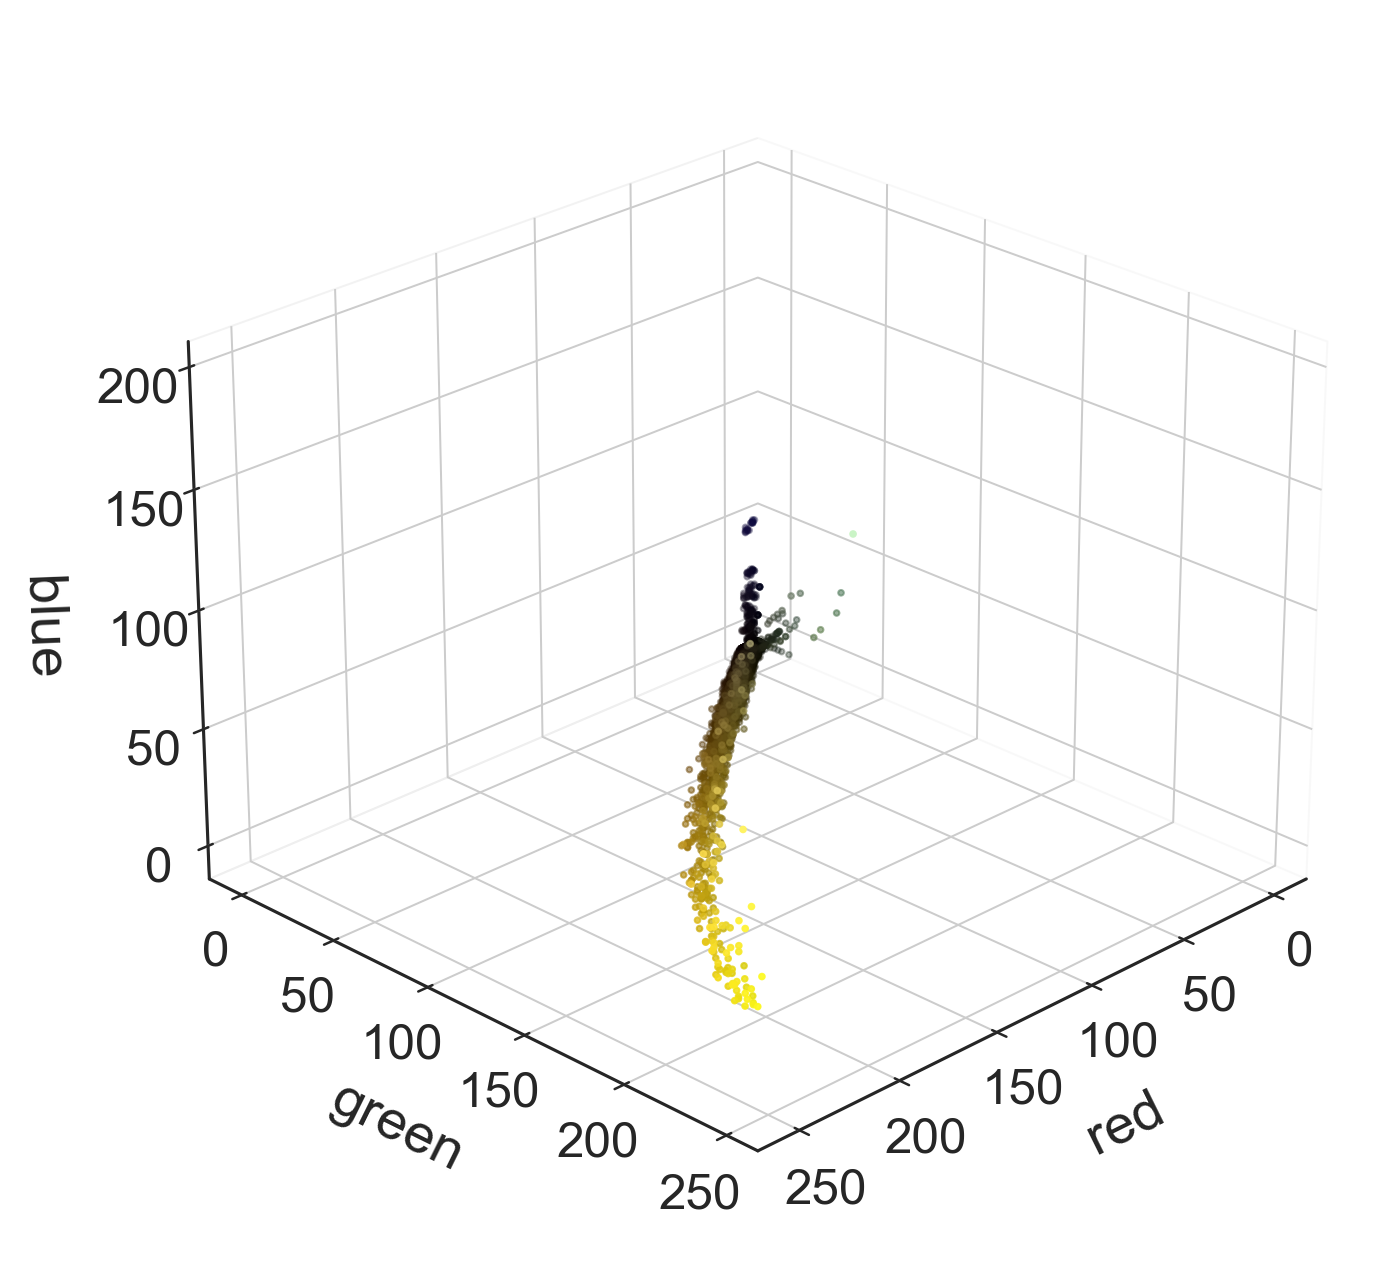
\includegraphics[width=0.55\textwidth]{figures/120_dataset/RGB_Mar21bS1C1R3_VLPAGl_200x_y.png}\label{fig:dataset:colorspace:rgb2}
    }
    \subfloat[HSV]{
    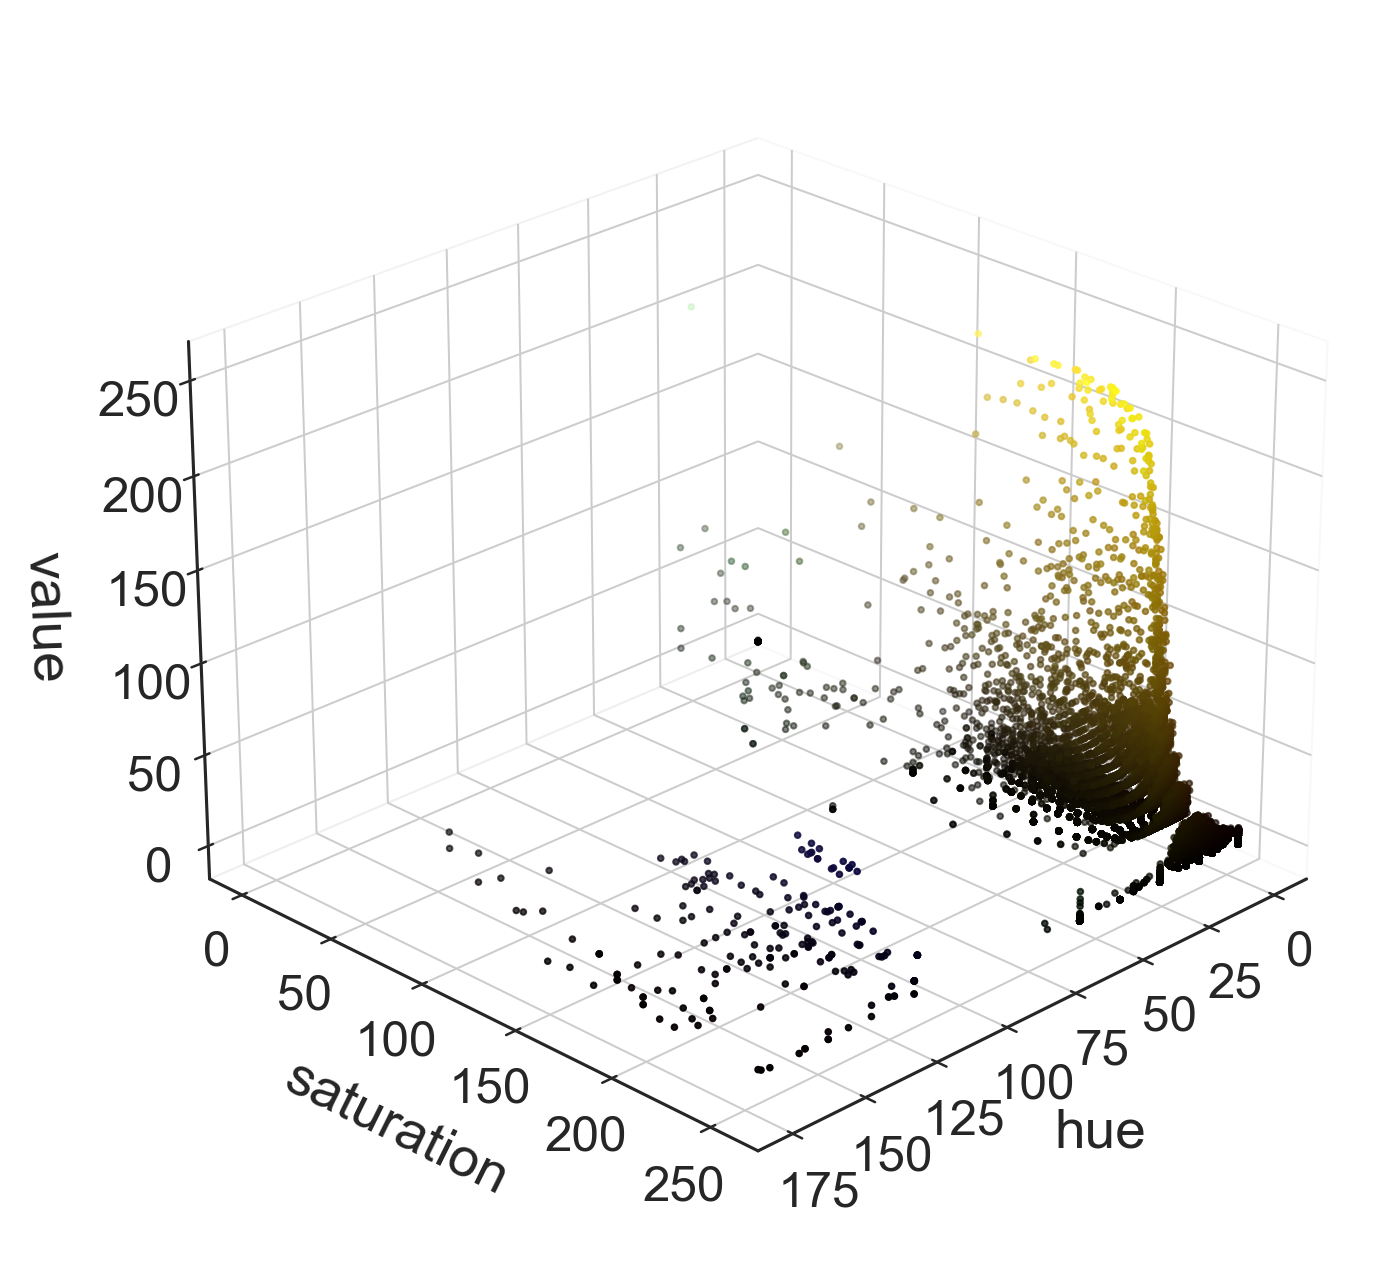
\includegraphics[width=0.55\textwidth]{figures/120_dataset/HSV_Mar21bS1C1R3_VLPAGl_200x_y.png}\label{fig:dataset:colorspace:hsv2}
    }}
    \caption{\textbf{Colorspace.} Two images represented as 3D points according to their RGB (left) and HSV (right) encodings. 
    Each point is colored as the corresponding pixel in the original image
    % The point color is the same as the pixel's color in the original image.
    }
    \label{fig:dataset:colorspace}
\end{figure}

% \clearpage
% \restoregeometry